%%%%%%%%%%%%%%%%%%%%%%%%%%%%%%%%%%%%%%%%%%%%%%%%%%%%%%%%%%%%%%%%%%%%%%%%%%%%%%%%
%2345678901234567890123456789012345678901234567890123456789012345678901234567890
%        1         2         3         4         5         6         7         8

% \documentclass[letterpaper, 10 pt, conference]{ieeeconf}  % Comment this line out if you need a4paper

\documentclass[a4paper, 10pt, conference]{ieeeconf}      % Use this line for a4 paper

\IEEEoverridecommandlockouts                              % This command is only needed if 
                                                          % you want to use the \thanks command

\overrideIEEEmargins                                      % Needed to meet printer requirements.

%In case you encounter the following error:
%Error 1010 The PDF file may be corrupt (unable to open PDF file) OR
%Error 1000 An error occurred while parsing a contents stream. Unable to analyze the PDF file.
%This is a known problem with pdfLaTeX conversion filter. The file cannot be opened with acrobat reader
%Please use one of the alternatives below to circumvent this error by uncommenting one or the other
%\pdfobjcompresslevel=0
%\pdfminorversion=4

% See the \addtolength command later in the file to balance the column lengths
% on the last page of the document

% The following packages can be found on http:\\www.ctan.org
\usepackage{graphics}
%\usepackage{parskip} % for pdf, bitmapped graphics files
\usepackage{epsfig} % for postscript graphics files
\usepackage{mathptmx} % assumes new font selection scheme installed
\usepackage{times} % assumes new font selection scheme installed
\usepackage{amsmath} % assumes amsmath package installed
\usepackage{amssymb}  % assumes amsmath package installed
\usepackage{float}
\usepackage{subcaption}
\usepackage{caption}

\title{\LARGE \bf Implementation of biologically-inspired dynamical systems for movement generation: automatic real-time goal adaptation and obstacle avoidance}
\usepackage[colorinlistoftodos]{todonotes}

\author{Alan Gomez, Samuel Parra, and Brennan Penfold \\ {\small \textbf{Advisor:} Djordje Vukcevic}}
\setlength{\parskip}{0pt}

\begin{document}



\maketitle
\thispagestyle{empty}
\pagestyle{empty}


%%%%%%%%%%%%%%%%%%%%%%%%%%%%%%%%%%%%%%%%%%%%%%%%%%%%%%%%%%%%%%%%%%%%%%%%%%%%%%%%
\begin{abstract}
The control algorithms of current robotic manipulators are quite rigid in their operation, often following precomputed paths, which is unsuitable for uses in dynamic environments associated with assisting humans. This paper presents a method of combining two current methods of collision monitoring \cite{Khatib} and collision avoidance \cite{Hoffmann} to create a safer more robust control algorithm. The collision monitoring algorithm is extended to monitor distances from all arm links but could not be implemented with the chosen collision avoidance method. The final collision monitoring library is able to operate at $\sim$ 250Hz, but would benefit greatly from optimisations to self collision monitoring, and the change to a null-space control algorithm would allow for collision avoidance to be implemented in all links.


\end{abstract}


%%%%%%%%%%%%%%%%%%%%%%%%%%%%%%%%%%%%%%%%%%%%%%%%%%%%%%%%%%%%%%%%%%%%%%%%%%%%%%%%
\section{Introduction} %Brennan
% Background, motivation and state of the art

%Background ---------------
Humanoid robots and arm like manipulators have a great many current and potential, useful applications. Currently robotic manipulators are used in a range of manufacturing processes like painting and spot welding \cite{Fadalil}. Another great application of humanoid robotics is to help people who cannot help themselves, as a separate system, or as a prosthetic. Robotic prosthetics have been implemented previously, like Dean Kamen's Luke Arm \cite{Adee}, but the control of such device is limited. In human applications the control system used in areas like manufacturing cannot be just dropped into place, there are many considerations that are required from both the software and hardware perspectives. In manufacturing applications manipulators typically use precomputed trajectories for robustness and efficiency, but this is unsuitable in a human environment, where obstacles and goals are constantly on the move \cite{Hoffmann}. The current approach in prosthetics is to use a human controller to solve this problem, by adding a joystick in a shoe \cite{Adee} or another such interface, so the operator can directly control the movement of the arm. While this addresses the adaptable control issue, it can be quite taxing for the user, requiring a lot of concentration just to perform basic tasks. This solution is also not very viable for stand-alone assistant robots, the cost of training an operator would far outweigh the benefit of using a robot and operator instead of a single human nurse or assistant. \\

One solution to the control problem is to use dynamic movement primitives, which can be generated during the movement itself, allowing for real-time obstacle avoidance and goal changes. Previous approaches \cite{Janabi-Sharif} used were initially not able to handle moving goals, but improvements made by H. Hoffmann et al. \cite{Hoffmann} by applying a potential field method to the process overcame this limitation. The use of dynamic movement primitives in the potential field method also overcame the local minimum problem, that is typically inherent with potential fields. Hence this paper is the basis of the project. There are some limitations to this method the most significant being the representation of the obstacles and manipulator. The method presented by H. Hoffman et al.\cite{Hoffmann} only considers points in cartesian space, where other methods, like those discussed by O. Khatib \cite{Khatib}, represent objects as basic primitives with volume and shape. \\

For objects to be avoided first they must be located relative to the manipulator, and that is the core concept of the library built for this project. Biologically-inspired dynamical systems for movement generation \cite{Hoffmann} does not tackle the problem of distances between objects, instead a precursor paper was used, Real-Time Obstacle Avoidance for Manipulators and Mobile Robots \cite{Khatib}. This paper goes into details on how to find the distance between two obstacles, which was modified to find the shortest vector between the two obstacles, allowing for it to be applied to the dynamic movements primitives control algorithm discussed by H. Hoffmann et al. \cite{Hoffmann}. These two techniques, along with the addition of distance monitoring with all links, has the potential to produce a better algorithm. The combination of the two techniques means that both the volume of the object is considered, and the trajectory planning can occur online allowing it to be adapted to any changes in a fast, efficient manner. These properties along with the addition of obstacle distance calculations for all links means that humanoid robots and manipulators would be more robust and safer to use in dynamic, human environments.
%Robotic assistants

\section{Approach}

\subsection{Distance to objects} %Alan
To compute the closest distance between two objects we first obtain the closest points between the objects, and then the distance between these two points. Since each shape is different in its mathematical representations, there is a unique case to consider for each combination of shapes, and these are as follows:

1) Between two spheres: 
To compute the closest distance between two spheres, one can just subtract the radius of the spheres from the distance between the center points of the spheres. The distance between the sphere center points can be easily calculated by finding the norm of the vector subtraction between the two center points. Since the norm of the vector is taken, the order of the vector subtraction does not matter.

2) Between a sphere and a capsule:
To compute the closest distance between a capsule $C$ and a sphere $S$, one can compute the distance between the center of the sphere, $p_S$, and the axis of symmetry of the cylinder, $l_C$
and then subtract the radius of the sphere and the capsule. 

The closest point, on $l_C$, to $p_S$ is given by \eqref{eq:capsule_point},

\begin{equation}       
    \begin{matrix} 
        x = x_1 + \lambda(x_2 - x_1) \\
        y = y_1 + \lambda(y_2 - y_1) \\
        z = z_1 + \lambda(z_2 - z_1) \label{eq:capsule_point}
    \end{matrix}
\end{equation}

where the start point of $l_C$ is $m1(x_1, y_1, z_1)$, the end point is $m2(x_2, y_2, z_2)$, and $\lambda$ is given by \eqref{eq:lambda}.

\begin{equation}       
    \begin{matrix} 
        \lambda = \frac{(c - m_1) \cdot (m_2 - m_1 )}{l^2} \label{eq:lambda}
    \end{matrix}
\end{equation}

3) Between two capsules:
To compute the closest distance between two capsules (capsule $A$ and capsule $B$), with axis of symmetry $l_A = \overline{m1_A m2_A}$ and $l_B = \overline{m1_B m2_B}$, 
where $A$ is the longest capsule, one can consider four different cases:
\begin{enumerate}
    \item $m1_B$ and $m2_B$ can be perpendicularly projected onto $l_A$
    \item $m1_B$ and $m2_B$ cannot be perpendicularly projected onto $l_A$
    \item only $m1_B$ can be perpendicularly projected onto $l_A$
    \item only $m2_B$ can be perpendicularly projected onto $l_A$
\end{enumerate} 

Depending on these cases, the following steps are going to be calculated with different objects.

In case 1, capsule $M$ will be capsule $A$, and capsule $O$ will be capsule $B$.

In case 2, if $m1_B$ is closer to $l_A$ than $m2_A$ is to $l_B$, then capsule $M$ will be capsule $A$, and capsule $O$ will be capsule $B$.
Else capsule $M$ will be capsule $B$, and capsule $O$ will be capsule $A$.

In case 3, if $m2_B$ is closer to $l_A$ than $m1_A$ is to $l_B$, then capsule $M$ will be capsule $A$, and capsule $O$ will be capsule $B$.
Else capsule $M$ will be capsule $B$, and capsule $O$ will be capsule $A$.

In case 4, if if $m1_B$ is closer to $l_A$ than $m2_B$ is to $l_A$, then capsule $M$ will be capsule $A$, and capsule $O$ will be capsule $B$.
Else capsule $M$ will be capsule $B$, and capsule $O$ will be capsule $A$.

With capsule $M$ and capsule $P$, one can follow the next steps.
The first step is to place the reference frame of $M$ in its center of mass, with the Z-axis in the direction of $l_M$. 
The second step is to project $l_O$ onto the XY-plane given by the reference frame of $M$ (Figure \ref{fig:capsule_capsule}),
the result of this projection would be the line $l_P$.
The third step is to calculate the closest point on $l_P$ to the origin of the reference frame of $P$ by using \eqref{eq:capsule_point}. 
The final step is to compute the distance and subtract the radius of the capsule and the sphere.
If the true closest points on the original axis of symmetry of the capsules are needed, one can project back the obtained points.

\begin{figure}[H]
    \centering
    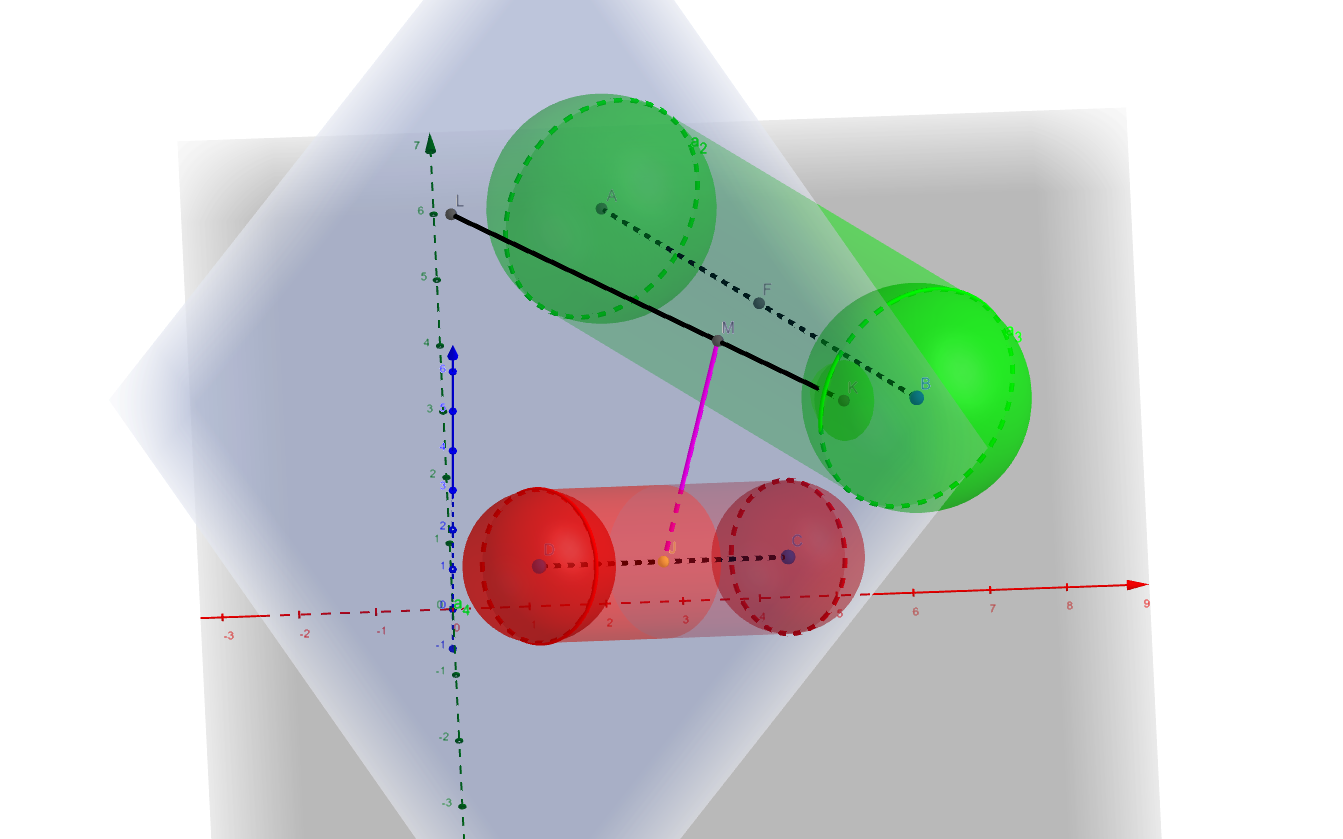
\includegraphics[scale=0.15]{images/capsule-capsule.png}
    \caption{Capsule - capsule}
    \label{fig:capsule_capsule}
\end{figure}


\subsection{Potential field} %Sam

To avoid collisions we decided to implement the method presented by Hoffmann et al. \cite{Hoffmann}. This method is based on dynamic movement primitives (DMP), which are used to generate a trajectory $x(t)$ with a velocity $v(t)$. These DMP are motivated from the dynamic of damped spring and can generate trajectories in many dimensions. These can be used to describe accelerations in 3D space that move towards a goal:

\begin{equation} \label{eq:1}
	\dot{v} = K ( g - x ) - D v - K (g - x_0) s + K f(s) + p(x, v)
\end{equation}

Where $g$ is the goal, $x$ is the current position, $x_0$ is the starting position, $v$ is the current velocity, $s$ is the phase variable, $D$ is the damping constant, and $K$ is the spring constant. The function $f(s)$ is a non-linear function used to define a learned path for the manipulator to take. However, the terms dependent on $s$ are not relevant for our application; thus we decided to not include it in the final equation.  

The last term is the potential field generated by the obstacles. This term has a repel effect on the end effector, making it avoid obstacles. The potential field is calculated as follow: We first determine the steering angle $\varphi$ using equation \ref{eq:2}, which is the angle between the velocity vector and a vector from the end effector to the obstacle as seen in Figure \ref{steering_image}. In our implementation, this vector is the shortest distance between the end-effector and the obstacle, as the original method considered points instead of volumes.


\begin{figure}
	\centering
	\scalebox{0.55}{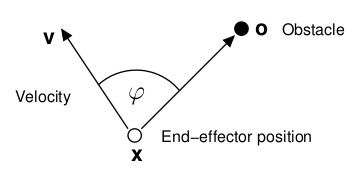
\includegraphics{images/steering_angle.png}}
	\caption{Graphical representation of steering angle \cite{Hoffmann}}
	\label{steering_image}
\end{figure}

\begin{equation} \label{eq:2}
	\varphi = cos^{-1} ((o-v)^T v / (\|o-x\| \cdot \|v\|));
\end{equation}

This steering angle determines how sharp the end effector steers away from the obstacle. The closer the angle is to 0, the more abrupt is the change of direction. The potential field is given by:

\begin{equation}
	p(x, v) = \gamma \sum_i R_i v \varphi_i exp(-\beta \varphi_i) 
\end{equation}

Where $\gamma$ and $\beta$ are tune-able constants, and R is a rotation matrix which rotates by the axis $r = (o-x) \times v $ with an angle of rotation of $\pi/2$. This rotation matrix can be calculated with the Rodrigues' rotation formula \cite{rodrigues}. The final potential field is the sum of the potential fields generated by all the obstacles. Our final equation converges towards the goal avoiding the obstacles in its way.

\begin{equation}
\dot{v} = K ( g - x ) - D v + p(x, v)
\end{equation}

\begin{figure*}[t]
	\centering
	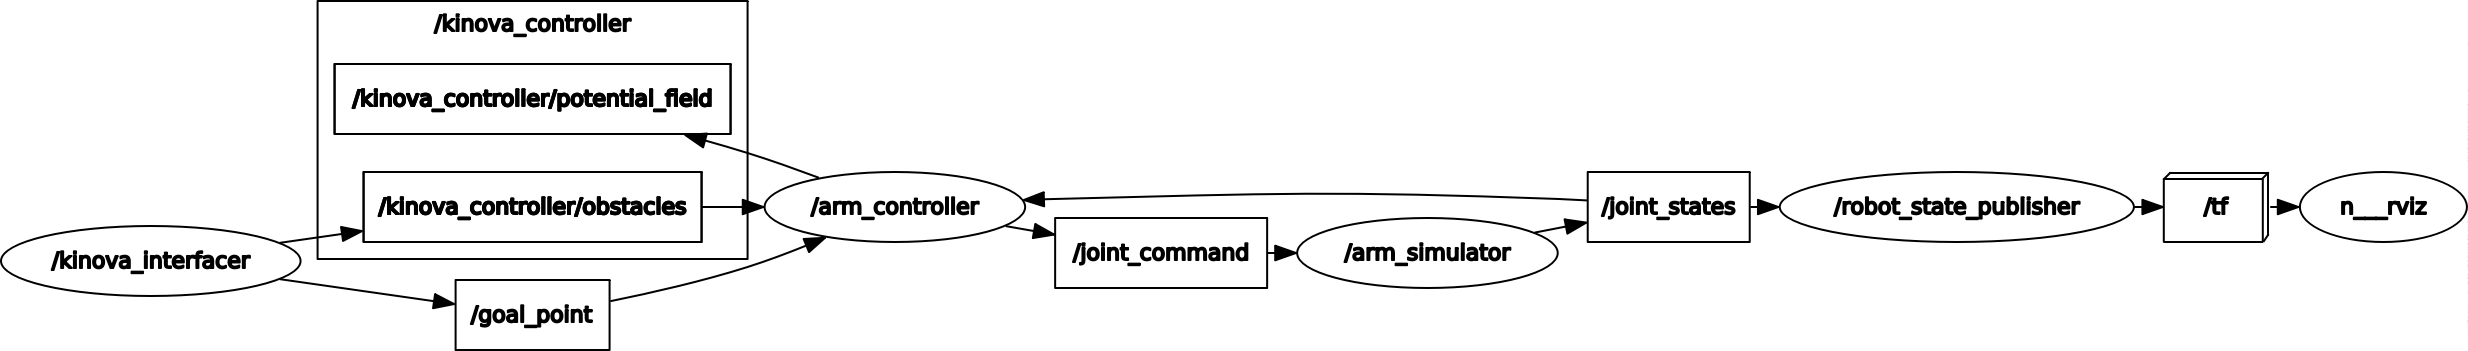
\includegraphics[scale=0.25]{images/rosgraph_single.png}
	\caption{ROS node graph for single arm}
	\label{fig:rosgraph_single}
\end{figure*}

\subsection{Collision monitoring library} %Sam

Our library was designed to be platform and framework independent. To achieve this, the library user must implement the Arm interface. This provides the flexibility of choosing how to describe mathematically the manipulator and update its position. Consider the case of two developers, one wants to use KDL for the forward and backwards kinematics, while the other one wants to derive the equations manually for a closed form solution. Both developers are supported by this library. 

In order to monitor the distances from the links of the arm to the obstacles in the workspace we represent the geometry of the links with the use of capsules. This representation enables us to calculate the distances between the links themselves in order to monitor self-collisions along with regular obstacles. This requires that the developer updates the geometric representation alongside the arm’s movement in the Arm implementation. 

\subsection{Controller} %Sam

The manipulator is controlled with a control loop that is executed at a specified rate. This loop is responsible for updating the geometric representation to match the real life manipulator and calculate the new velocity with the collision avoidance algorithm. In the loop the developer must keep the current position, velocity, positions of obstacles, and goal updated for the algorithm to produce an accurate output. 
 
 
\section{Implementation} %Brennan
The final product that combines all the obstacle monitoring and avoidance techniques was implemented using the Robotic operating system (ROS) framework, specifically ROS Kinetic. ROS has a few advantages in this area, the first and foremost being the Kinova Kortex library \cite{kortex}, which is a high and low level control API for Kinova robotic manipulators, including the one chosen for demonstration. This library has a lot of useful features from the MoveIt control algorithm to the fully fledged gazebo simulation of the arm. The final software produced does actually rely on any of the Kortex libraries, but was instrumental in testing and development. \\

The ROS package can be broken down into 3 sections, the controller, simulator and visualisation. The control section is the implementation of Biologically-inspired dynamical systems for movement generation \cite{Hoffmann}, the collision avoidance library is implemented inside a control loop that uses the monitor class to obtain the shortest distance vectors from the obstacles to the end-effector. This shortest distance is then passed into the potential field method along with the current velocity of the manipulator. From this the new velocity is derived and then passed into the simulator via an inverse kinematics function of the KinovaArm class, mapping the velocity from cartesian space to the manipulators joint space. \\

The simulation software takes the joint velocities from the controller and updates the current state of the simulated manipulator, and then passes the current state back to the controller as well as forwards to the visualisation. The simulation algorithm it's self is very basic and is based around a discrete time integration technique:
$$
\theta_i = \theta_{i-1} + \dot{\theta}_{i-1}\times (t_i - t_{i-1})
$$ 
While rudimentary, as it doesn't consider inertia or any other complex parameters, it functions as desired for the testing and demonstration of a robotic manipulators trajectory control algorithm. \\

The basic ROS node graph can be seen in figure \ref{fig:rosgraph_single} where the interfacer is a basic terminal interface to send goals to the arm controller and the visualisation is performed by the built-in robot\_state\_publisher node and Rviz.


\section{Experiments}

\subsection{Collision Monitoring} %Brennan
The collision monitoring library has no practical measure of accuracy because of its pure mathematical basis. To assert the accuracy of the mathematics applied the distance between objects was verified using Geogebra models, and the rest of the software relies on those calculations. So the core performance measure of the collision monitoring library can be considered speed, hence the use of C++ instead of a higher level interpreted language like python. The performance test was performed on an Ubuntu 16.04 machine with a Intel Core i5-7200U 2.5GHz CPU. The following operations were timed using the C++ chrono library:
\begin{itemize}
	\item The joint initialisation of one KinovaArm and Monitor class.
	\item The combination of initialising a Sphere and adding it to the Monitor class.
	\item The updatePose function, which updates the internal kinematic representation of the arm.
	\item The distanceToObjects function, calculating the distance from each of the manipulators links to the obstacle.
	\item The distanceBetweenArmLinks function, measuring the distance from each of the links to the other links in the same manipulator.
\end{itemize}

\subsubsection{Results}
Each operation was performed 100 times with a single spherical obstacle and mean calculated to produce the final results given in Table \ref{table:Function Times} below.

\begin{table}[H]
	\centering
	\begin{tabular}{|l|l|}
		\hline
		Operation & Time (seconds) \\ \hline
		Init arm and monitor   & 0.00103831     \\ \hline
		Init and add object    & 0.00000276     \\ \hline
		Update the arm position& 0.00012871     \\ \hline
		Distance to obstacle   & 0.00026022     \\ \hline
		Distance to self links & 0.00199209     \\ \hline
	\end{tabular}
	\caption{Execution times for collision monitoring tasks}
	\label{table:Function Times}
\end{table}
From a cursory glance it is clear that the functions are quite fast, all operations take less than two milliseconds to complete, but some of the operations are not as fast as desired. From a runtime perspective the initialisation operations are not that important when is comes to overall speed, since they tend to only be run at the start of the program, and potentially at random intervals the program in the case of the obstacle initialisation. The distance to obstacles, distance between arm links, and the update function are the main operations relevant to the software refresh rate, these run every loop and depict the final update rate of the software. The update function of the arm is very fast, and the distance to obstacles function is the same only taking twice as long. It is important to note though that the time for distance to obstacles to execute relies on the number of obstacles, as the number of obstacles increases so does the time to calculate, in a linear fashion. This means that with 40 obstacles the software will be restricted to $\sim$ 10Hz. Assuming only one obstacle the other large impact to overall performance in the distance to self links operation, taking up over four times the time used by the other two core functions combined. This was somewhat expected, if not to this extent, since the software was designed for portability in mind, which limits the possible optimisations available, still further investigation into the limiting factors should be performed. The final core loop time for the collision monitoring library is a little over 4.7 milliseconds, which would give a update rate of $\sim$ 250hz, but this would gain significant benefits from the exclusion of the distance to own links monitoring functions.



\subsection{Single arm obstacle avoidance} %Sam
% In order to visualize the obstacle avoidance we first simulated a single instance of the Kinova\textsuperscript{\tiny\textregistered} Gen3 robotic manipulator and placed obstacles in its workspace, as seen in Fig. \ref{fig:one_arm}. We then provided different commands to find tune the relevant parameters and assess the effectiveness of the algorithm. 
 To assess the effectiveness of the algorithm we place several obstacles in the vicinity of the manipulator, and then command it to move between points in the workspace. First, we used the same set of obstacles, initial point and goal point for two experiments with two different values for $\gamma$ as seen in Figure 4. When $\gamma=0$ there is no influence of the potential field in the velocity, hence the end effector does not avoid the obstacle. Whereas when $\gamma=35$ the effect of the potential field steers the end effector away from the obstacle in its path. From these results we can assess that the DMP will converge to the goal point, and the value of $\gamma$ has an impact in the effectiveness of the algorithm. 

\begin{figure}[H]
	\centering
	\label{potential}
	\begin{subfigure}[t]{0.20\textwidth}
		\centering
		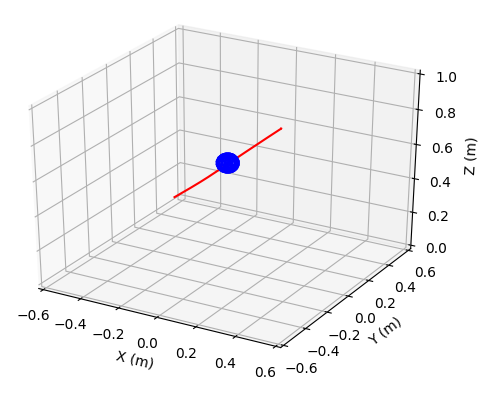
\includegraphics[scale=0.35]{images/no_potential.png}
		\caption{$\gamma = 0$}
	\end{subfigure}%
	~ 
	\begin{subfigure}[t]{0.20\textwidth}
		\centering
		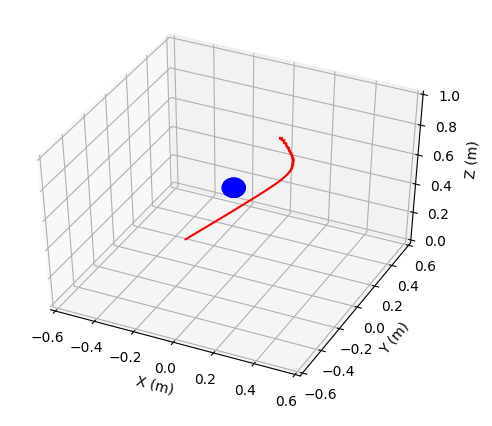
\includegraphics[scale=0.35]{images/yes_potential.png}
		\caption{$\gamma = 35$}
	\end{subfigure}
	\caption{Movement with different values for $\gamma$}
\end{figure}

In Figure \ref{fig:potential_field} we can observe the behaviour of the potential field when several obstacles are nearby. Note that the potential field's magnitude is larger when the end effector is approaching the obstacles and gets smaller after it passes the obstacles. This is the effect of the steering angle, as when the end effector passes the obstacles the angle between the current velocity and the obstacles is large. It should also be noted that the direction of the potential field effect is not uniform between small steps.

\begin{figure}[H]
	\centering
	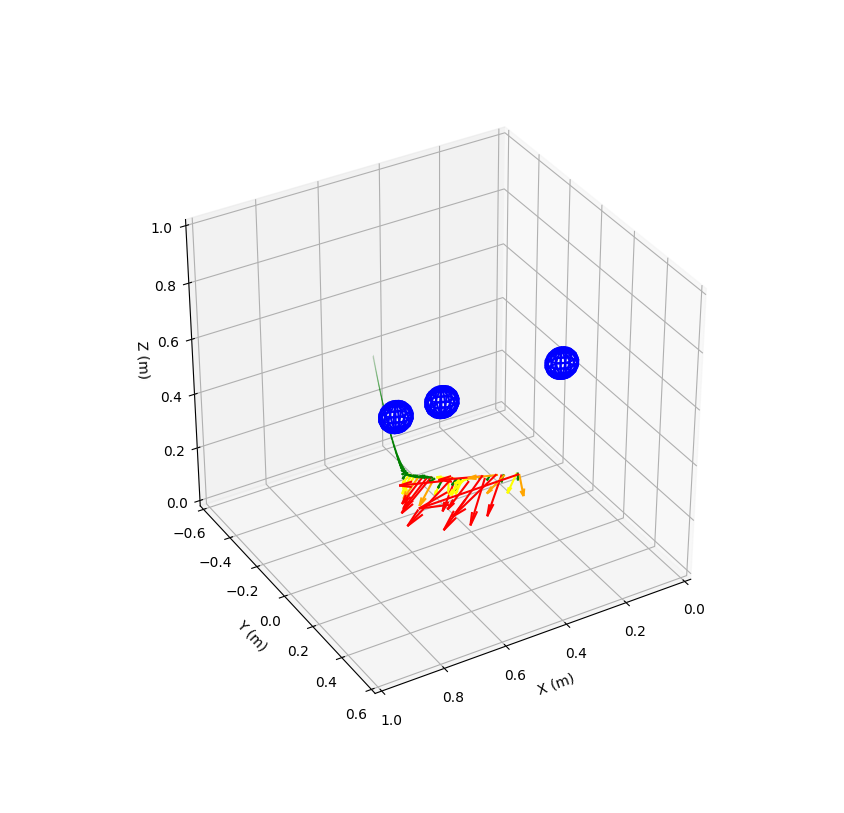
\includegraphics[scale=0.30]{images/potential_field.png}
	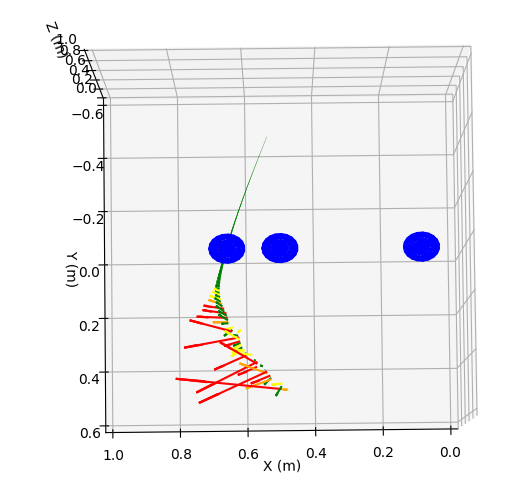
\includegraphics[scale=0.30]{images/potential_field_top.png}
	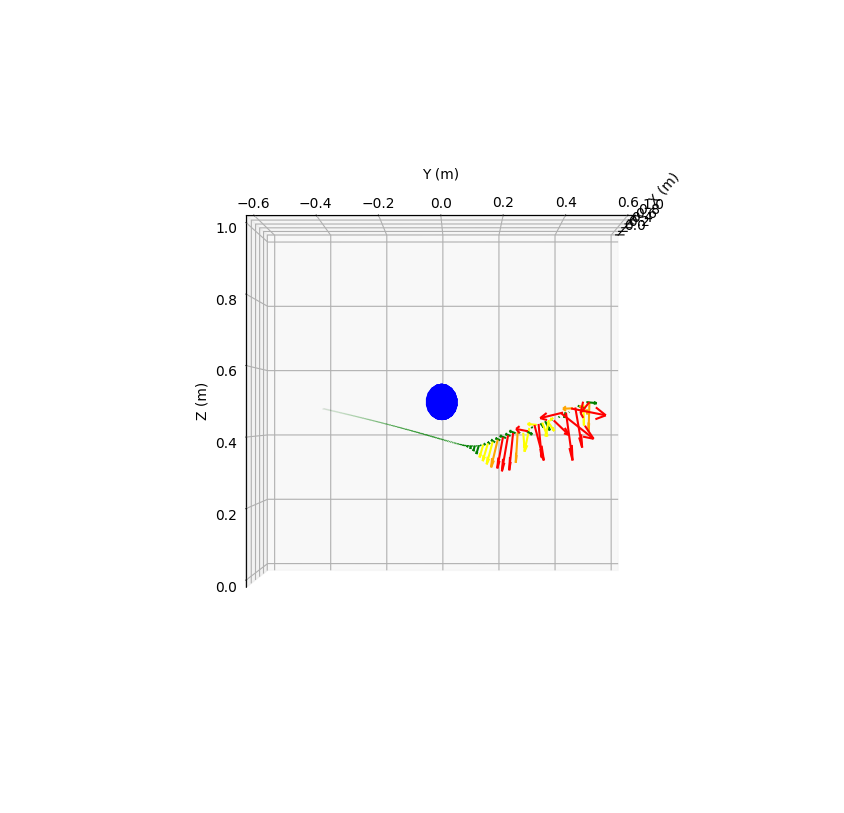
\includegraphics[scale=0.30]{images/potential_field_side.png}
	\caption{Potential field generated during the movement}
	\label{fig:potential_field}
\end{figure}
\pagebreak
For one of the experiments we placed several obstacles in the workspace and command it to move between points. The results of the collision avoidance algorithm can be seen from several perspectives in fig \ref{fig:one_arm_avoidance}. The red line is the path of the end effector from the initial point to the goal. In fig \ref{fig:one_arm_avoidance_vector} the velocity vectors in their respective point in time can be observed. 

\begin{figure}[H]
	\centering
	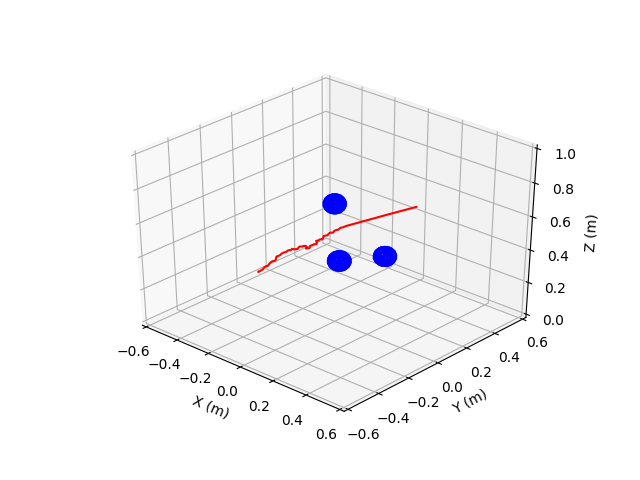
\includegraphics[scale=0.30]{images/one_arm_three_obstacles.png}
	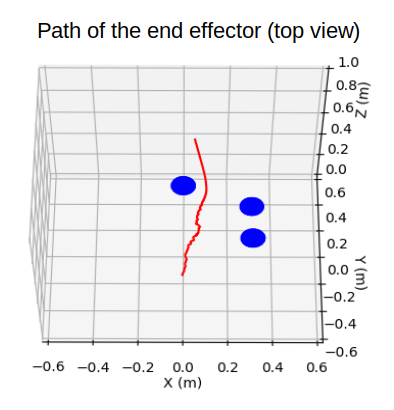
\includegraphics[scale=0.30]{images/one_arm_three_obstacles_top.png}
	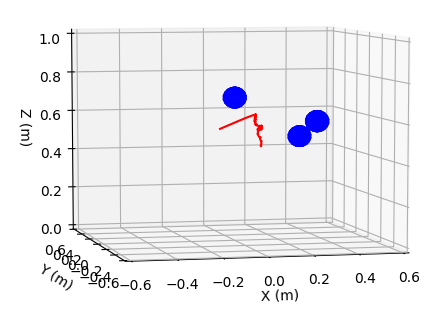
\includegraphics[scale=0.30]{images/one_arm_three_obstacles_side.png}
	\caption{Path of the end effector as it moves through obstacles}
	\label{fig:one_arm_avoidance}
\end{figure}

\begin{figure}[H]
	\centering
	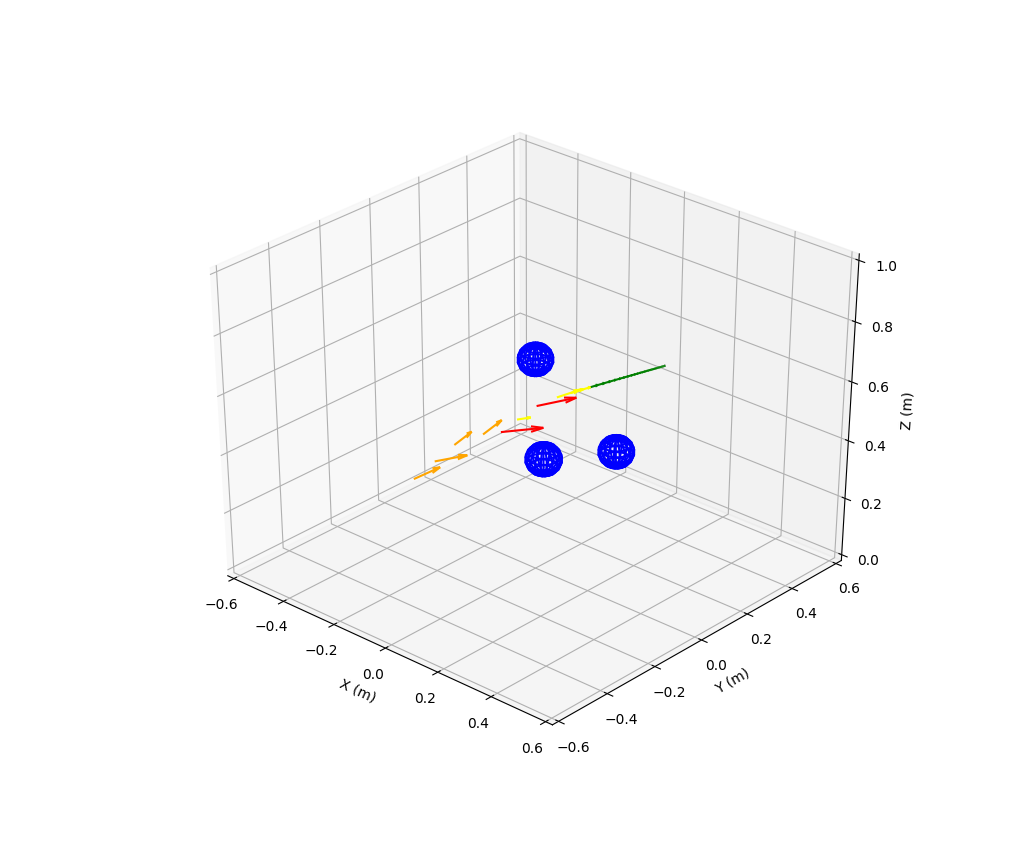
\includegraphics[scale=0.30]{images/one_arm_three_obstacles_vector.png}
	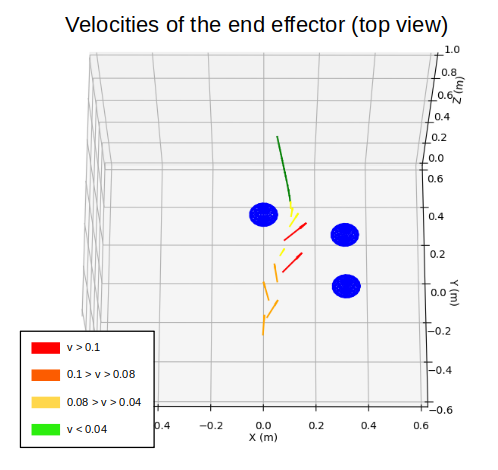
\includegraphics[scale=0.30]{images/one_arm_three_obstacles_top_vector.png}
	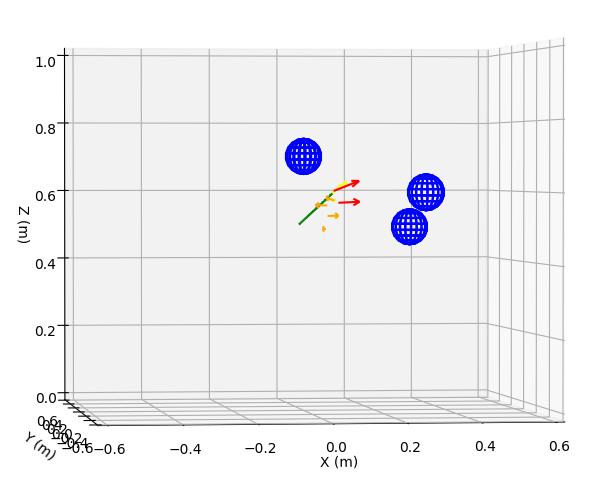
\includegraphics[scale=0.30]{images/one_arm_three_obstacles_side_vector.png}
	\caption{Cartesian velocities generated by the algorithm}
	\label{fig:one_arm_avoidance_vector}
\end{figure}

As it can be observed from Figure \ref{fig:one_arm_avoidance} and Figure \ref{fig:one_arm_avoidance_vector} the collision avoidance algorithm can generate velocities that avoid several obstacles without problems. 

\subsection{Dual arm collision avoidance} %Sam

In order for two manipulators to operate with intersecting workspaces it is important that they do not collide with each other. In this experiment we simulated two instances of the Kinova arm placed close to each other so their workspaces would overlap. Each arm is individually controlled, meaning we could place one arm on the path of the other to assess if the arms avoided collisions. An example setup can be seen in Figure \ref{fig:two_arms}. The objective is to assess if the arms avoid colliding with each other during operation.

\begin{figure}[H]
	\centering
	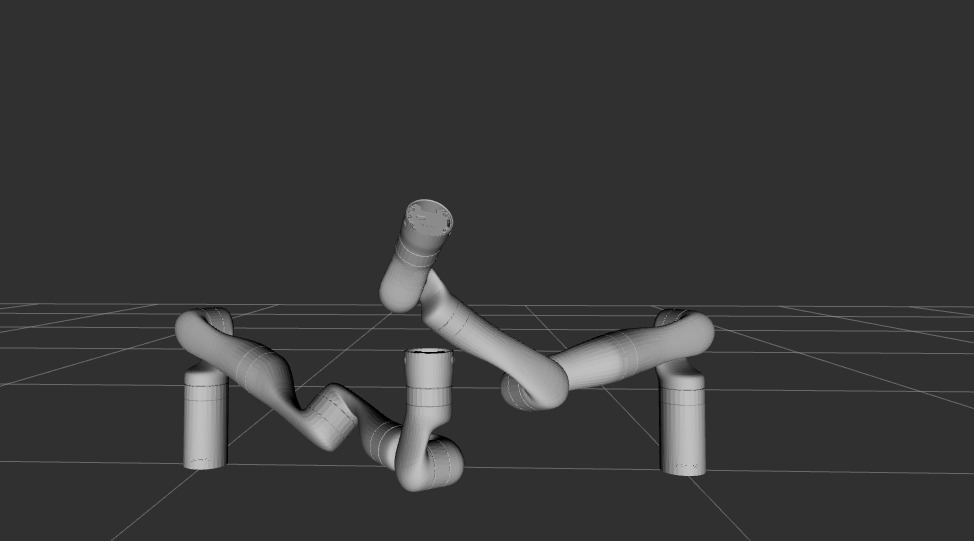
\includegraphics[scale=0.15]{images/two_arms.jpeg}
	\caption{Two arms sharing a space}
	\label{fig:two_arms}
\end{figure}

In Figure \ref{fig:two_arm_avoidance} the path of the end effector of first Kinova arm can be seen as well as the pose of the second arm. The pose of the second arm remained constant during the movement of the first arm. 

\begin{figure}[H]
	\centering
	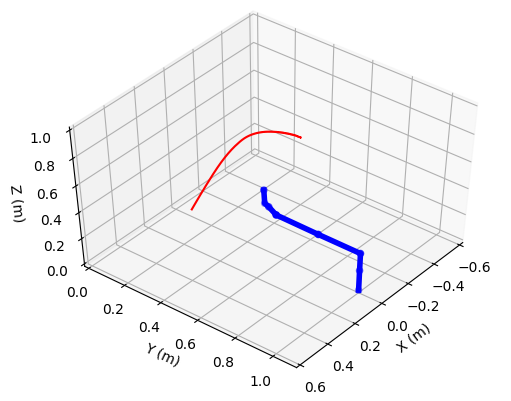
\includegraphics[scale=0.25]{images/two_arms.png}
	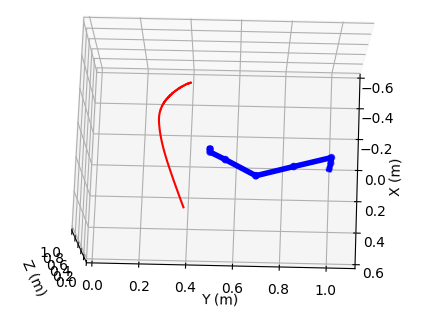
\includegraphics[scale=0.25]{images/two_arms_top.png}
	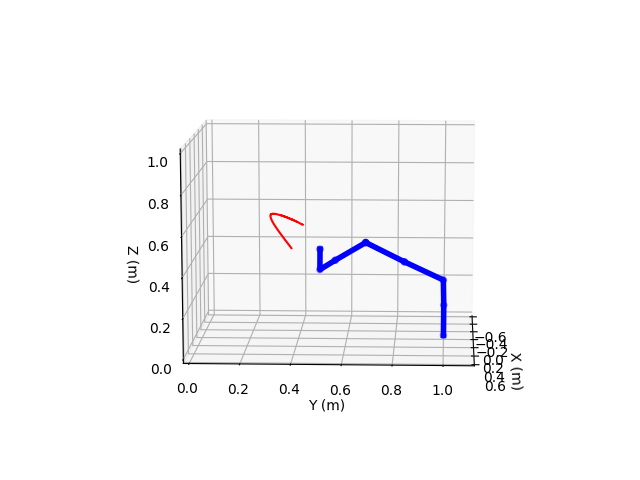
\includegraphics[scale=0.25]{images/two_arms_side.png}
	\caption{Path of the end effector of one arm}
	\label{fig:two_arm_avoidance}
\end{figure}

\begin{figure}[H]
	\centering
	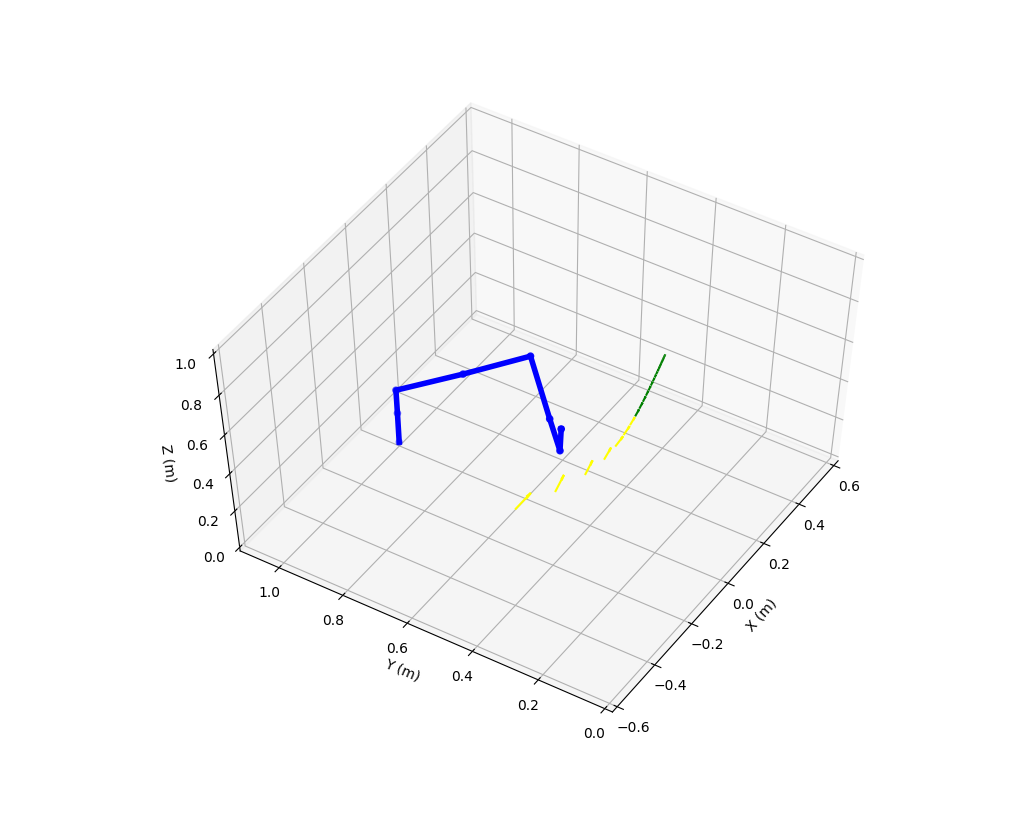
\includegraphics[scale=0.25]{images/two_arms_vector.png}
	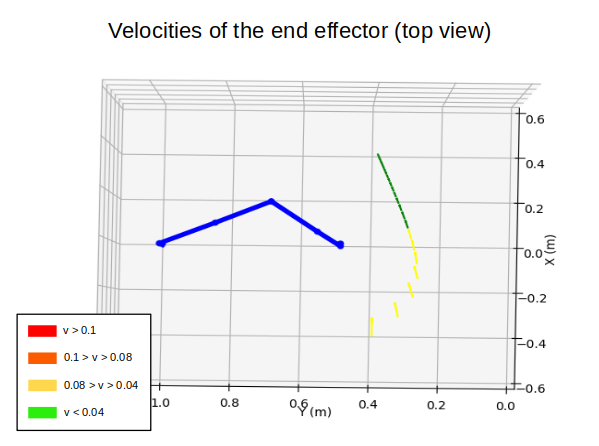
\includegraphics[scale=0.25]{images/two_arms_vector_top.png}
	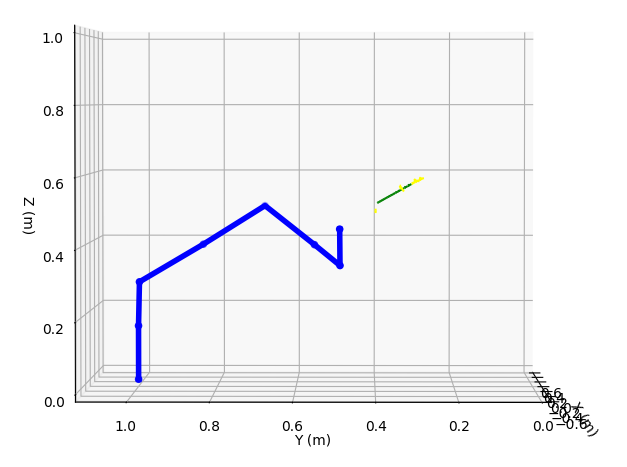
\includegraphics[scale=0.25]{images/two_arms_vector_side.png}
	\caption{Cartesian velocities generated}
	\label{fig:two_arm_avoidance_vector}
\end{figure}
\pagebreak
From these results we can see that a long as the geometric representation of the two arms is accurate, the collision avoidance algorithm can be use to avoid collisions between the arms. The collision avoidance algorithm only monitors the end effector of the moving robot, this means that not all collision between the two arms can be avoided. To fix this a null space control algorithm would need to be implemented. 

\section{Use cases}

\subsection{Single arm} %Alan
The library presented in this paper can be used with a single manipulator to avoid the collision of its end-effector with objects in the environment.
The user can use the Arm interface to provide the necessary information about the manipulator.
The user can then also add different obstacles that are present in the environment.
The pose of the manipulator and the obstacles need to be updated using the methods given by the library.
\subsection{Dual arm} %Alan
The user can also use the library with two manipulators by creating two instances of the implementation of the Arm interface and adding the links of 
the opposite manipulator as obstacles represented by capsules.
This will prevent the collision of the end-effector of both robots with the opposite manipulator
\subsection{Multiple arms}
In the same way, the library can be used with more than two manipulators. The user can add as many manipulators as the computational resources allow.
\subsection{Self collision} %Alan
Finally, a user can also use this library to prevent the collision of the end-effector of the manipulator with its other links.
This can be done by implementing the Arm interface and adding each link of the robot as an obstacle represented by a capsule.

\section{Conclusion}
For robotic manipulators to be used in a human environment they first need to have the ability to adapt in constantly changing, dynamic environments. This can be done in a robust and safe manner using a combination of two different methods discussed by H. Hoffmann et al. \cite{Hoffmann} and O. Khatib \cite{Khatib}. By implementing the obstacle monitoring by O. Khatib \cite{Khatib} and the collision avoidance by H. Hoffmann et al. \cite{Hoffmann}, along with monitoring collisions for all links, robotic manipulators are more resilient to changes in obstacle and goal placement. The final collision monitoring library can have an update rate of $\sim$ 200Hz with all features enabled, this is a viable update rate, but this would become drastically impacted if more that 10 obstacles were to be added to the environment. % Sam can sumarise about his results.
From the experiments it can be concluded that the DMPs used in this algorithm converge to the goal, and that the potential field term influences the end effector's path to steer away from obstacles. 
It can also be observed that the effectiveness of the algorithm is dependent on the parameters of the DMP equation, hence it is important for a developer to fine tune this parameters until a certain level of performance is reached.
 
While the algorithm produced gives some significant benefits over previous methods, there is still a lot of potential improvements. The collision monitoring library could benefit greatly from some optimisation of the self collision functions, along with the addition of more shapes. The current shapes are a basic sphere and capsule, with the addition of an n-ellipsoid primitive a large majority of basic shapes and structures could be constructed by the combination of the primitives. % Sam can add any future works given from his section or results.
Finally, in order to avoid more serious collisions, the algorithm should consider the entire body of the manipulator rather than just the end effector. 

%The computation of the distances between different kinds of objects is not easy, one needs to take into consideration different scenarios, otherwise, the main algorithm might fail. Further work on this area could be adding other kinds of shapes.


\addtolength{\textheight}{-12cm}   % This command serves to balance the column lengths
                                  % on the last page of the document manually. It shortens
                                  % the textheight of the last page by a suitable amount.
                                  % This command does not take effect until the next page
                                  % so it should come on the page before the last. Make
                                  % sure that you do not shorten the textheight too much.

%%%%%%%%%%%%%%%%%%%%%%%%%%%%%%%%%%%%%%%%%%%%%%%%%%%%%%%%%%%%%%%%%%%%%%%%%%%%%%%%



%%%%%%%%%%%%%%%%%%%%%%%%%%%%%%%%%%%%%%%%%%%%%%%%%%%%%%%%%%%%%%%%%%%%%%%%%%%%%%%%



%%%%%%%%%%%%%%%%%%%%%%%%%%%%%%%%%%%%%%%%%%%%%%%%%%%%%%%%%%%%%%%%%%%%%%%%%%%%%%%%
\section*{Acknowledgements}
We would like to thank our supervisor Djordje Vukcevic for all the advice and help this semester.

%%%%%%%%%%%%%%%%%%%%%%%%%%%%%%%%%%%%%%%%%%%%%%%%%%%%%%%%%%%%%%%%%%%%%%%%%%%%%%%%


\begin{thebibliography}{10}
	
\bibitem{Khatib} O. Khatib, “Real-Time Obstacle Avoidance for Manipulators and Mobile Robots” The International Journal of Robotics Research, vol. 5, no. 1, pp. 90–98, Mar. 1986, doi: 10.1177/027836498600500106.
\bibitem{Hoffmann} H. Hoffmann, P. Pastor, D.-H. Park, and S. Schaal, “Biologically-inspired dynamical systems for movement generation: Automatic real-time goal adaptation and obstacle avoidance,” in 2009 IEEE International Conference on Robotics and Automation, Kobe, May 2009, pp. 2587–2592, doi: 10.1109/ROBOT.2009.5152423.
\bibitem{Fadalil} M. S. Fadali and A. Visioli, “Introduction to Digital Control,” in Digital Control Engineering, Elsevier, 2013, pp. 1–8.
\bibitem{Adee} S. Adee, “Dean Kamen’s ‘Luke Arm’ Prosthesis Readies for Clinical Trials - IEEE Spectrum,” IEEE Spectrum: Technology, Engineering, and Science News, Feb. 01, 2008. https://spectrum.ieee.org/biomedical/bionics/dean-kamens-luke-arm-prosthesis-readies-for-clinical-trials (accessed Jun. 25, 2020).
\bibitem{Janabi-Sharif} F. Janabi-Sharifi and D. Vinke, “Integration of the artificial potential field approach with simulated annealing for robot path planning,” in Proceedings of 8th IEEE International Symposium on Intelligent Control, Aug. 1993, pp. 536–541, doi: 10.1109/ISIC.1993.397640.
\bibitem{rodrigues}  Belongie, Serge. "Rodrigues' Rotation Formula." From MathWorld--A Wolfram Web Resource, created by Eric W. Weisstein. https://mathworld.wolfram.com/RodriguesRotationFormula.html 
\bibitem{kortex} Kinovarobotics/ros\_kortex. Kinova Robotics, 2020.

%\bibitem{Velliste} M. Velliste, S. Perel, M. C. Spalding, A. S. Whitford, and A. B. Schwartz, “Cortical control of a prosthetic arm for self-feeding,” Nature, vol. 453, no. 7198, Art. no. 7198, Jun. 2008, doi: 10.1038/nature06996.



\end{thebibliography}


\end{document}
